\documentclass[tikz]{standalone}
\usepackage{pgfplots}
\usepgfplotslibrary{groupplots}
\pgfplotsset{compat=1.18}
\definecolor{utnblue}{RGB}{0, 102, 204}

\begin{document}
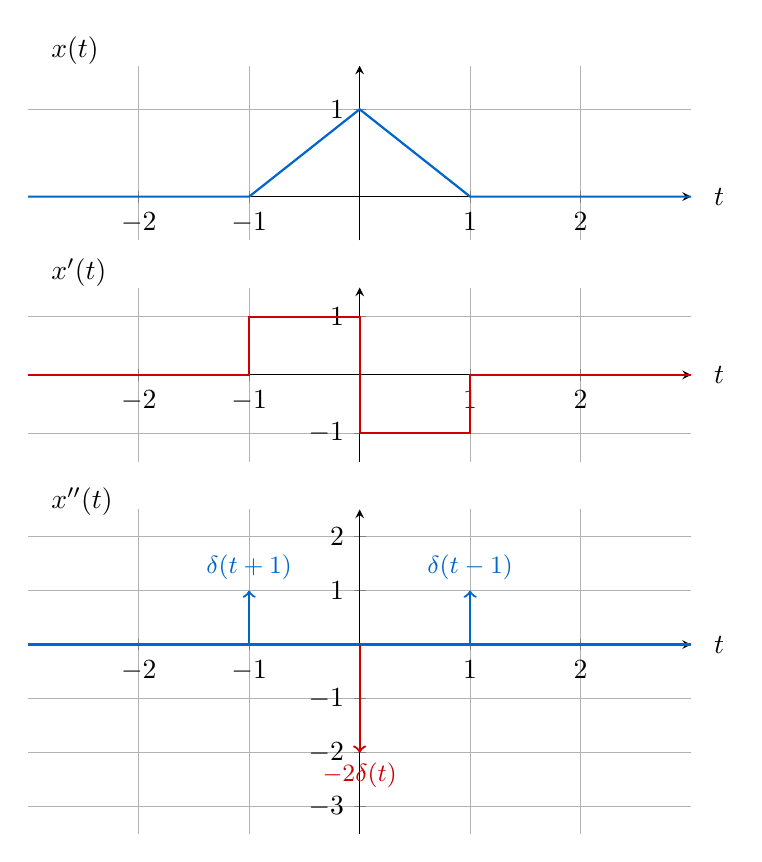
\begin{tikzpicture}
    \begin{groupplot}[
        group style={
            group size=1 by 3,
            vertical sep=0.6cm,
        },
        width=10cm,
        height=3.8cm,
        axis lines=middle,
        xmin=-3, xmax=3,
        grid=both,
        grid style={line width=.1pt, draw=gray!40},
        major grid style={line width=.2pt,draw=gray!60},
        xtick={-2,-1,0,1,2},
        every axis plot/.append style={thick},
        every axis x label/.append style={at={(ticklabel* cs:1.02)}, anchor=west},
        every axis y label/.append style={at={(rel axis cs:0.02, 0.95)}, anchor=south west, rotate=0},
    ]
    
    % Panel 1: x(t)
    \nextgroupplot[
        ymin=-0.5, ymax=1.5,
        ytick={0,1},
        ylabel={$x(t)$}, xlabel={$t$},
    ]
    \addplot[utnblue] coordinates {(-3,0) (-1,0) (0,1) (1,0) (3,0)};
    
    % Panel 2: x'(t)
    \nextgroupplot[
        ymin=-1.5, ymax=1.5,
        ytick={-1,0,1},
        ylabel={$x'(t)$}, xlabel={$t$},
    ]
    \addplot[red!80!black] coordinates {(-3,0) (-1,0) (-1,1) (0,1) (0,-1) (1,-1) (1,0) (3,0)};
    
    % Panel 3: x''(t) — impulsos
    \nextgroupplot[
        height=5.7cm,
        ymin=-3.5, ymax=2.5,
        ytick={-3,-2,-1,0,1,2},
        ylabel={$x''(t)$}, xlabel={$t$},
    ]
    % Nivel cero de la señal x''(t)
    \addplot[thick, utnblue] coordinates {(-3,0) (3,0)};
    % Impulsos como flechas
    \draw[->, thick, utnblue] (axis cs:-1,0) -- (axis cs:-1,1) node[above, font=\small] {$\delta(t+1)$};
    \draw[->, thick, red!80!black] (axis cs:0,0) -- (axis cs:0,-2) node[below, font=\small] {$-2\delta(t)$};
    \draw[->, thick, utnblue] (axis cs:1,0) -- (axis cs:1,1) node[above, font=\small] {$\delta(t-1)$};
    
    \end{groupplot}
\end{tikzpicture}
\end{document}
